\newcommand{\selector}[0]{[~S~\Rightarrow~y;~BE~] \lolli HE}
\newcommand{\comprehension}[0]{\{~\widehat{x};~BE;~SH~\}}
\newcommand{\aggregate}[0]{[~A~\Rightarrow~y;~\widehat{x};~BE;~SH_1;~SH_2~]}

%%%%%%%%%%%%%%%%%%%%%%%%%%%%%%%%%%%%%%%%%%%%%%%%%%%%%%%%%%%%%%%%%%%%%%

\section{The LM Language}
\label{lm_language}

Linear Meld (LM) is a logic programming language that offers a
declarative and structured way to manage mutable state.  A program consists of
a database of facts and a set of derivation rules. The database
includes persistent and linear facts. Persistent facts cannot be
deleted, while linear facts can be asserted and retracted.

The dynamic (or operational) semantics of LM is identical to
Datalog. Initially, we populate the database with the \emph{program's axioms} (initial facts)
and then determine which derivation rules can be applied by
using the current database. Once a rule is applied, new facts can be
derive, which are then added to the database. If a rule uses linear
facts, they are retracted from the database. The program stops when
\emph{quiescence} is achieved, i.e., when rules no longer apply.

Each fact is a predicate on a tuple of \emph{values}, where the type
of the predicate prescribes the types of the arguments.  LM rules are
type-checked using the predicate declarations in the header of the
program. LM has a simple type system that includes types such as
\emph{node}, \emph{int}, \emph{float}, \emph{string},
\emph{bool}. Recursive types such as \emph{list X} and \emph{pair X;
  Y} are also allowed.  Each rule in LM has a defined priority that is
inferred from its position in the source file.  Rules at the beginning
of the file have higher priority.
We consider all the new facts that have been not used yet to create a
set of \emph{candidate rules}.
The set of candidate rules is then applied (by priority)
and updated as new facts are derived.

%%%%%%%%%%%%%%%%%%%%%%%%%%%%%%%%%%%%%%%%%%%%%%%%%%%%%%%%%%%%%%%%%%%%%%

\subsection{Example}

\begin{figure}[t]
{\footnotesize
\begin{Verbatim}[numbers=right]
type left(node, node).
type right(node, node).
type linear value(node, int, string).
type linear replace(node, int, string).

// set of rules
replace(A, K, New),
value(A, K, Old)
   -o value(A, K, New). // we found our key

replace(A, RKey, RValue),
value(A, Key, Value),
!left(A, B),
RKey < Key
   -o value(A, Key, Value),
      replace(B, RKey, RValue). // go left

replace(A, RKey, RValue),
value(A, Key, Value),
!right(A, B),
RKey > Key
   -o value(A, Key, Value),
      replace(B, RKey, RValue). // go right

// initial configuration
!left(@0, @1).   !right(@0, @2).
!left(@1, @3).   !right(@1, @4). 
!left(@2, @5).   !right(@2, @6).

value(@0, 3, a).   value(@1, 1, b).
value(@2, 5, c).   value(@3, 0, d).
value(@4, 2, e).   value(@5, 4, f).
value(@6, 6, g).

// update key 6 to value x
replace(@0, 6, x).
\end{Verbatim}
}
\caption{LM program for replacing a key's value in a binary tree dictionary}
\label{code:btree_replace}
\end{figure}

We now present in Fig.~\ref{code:btree_replace}, a LM program that
implements the update operation for a binary tree dictionary
represented as key/value pairs. We first declare the predicates (lines
1-4) which represent the facts we are going to use. Predicate
\texttt{left/2} and \texttt{right/2} are persistent while predicates
\texttt{value/3} and \texttt{replace/3} are linear. Predicate
\texttt{value/3} assigns a key/value pair to a tree node and predicate
\texttt{replace/3} represents an update operation that updates the key
in the second argument to the value in the third argument.

The algorithm uses three rules for the three cases of updating a key's
value: the first rule performs the update (lines 6-9); the second rule
recursively picks the left branch for the update operation (lines
11-16); and the third rule picks the right branch (lines 18-23). The
initial axioms are presented in lines 26-33 and they describe the
initial binary tree configuration, including keys and values.
Finally, with the \texttt{replace(@0, 6, x)} axiom instantiated at the
root node $@0$, we intend to change the value of key 6 to value
`$x$'. Note that when writing rules or axioms, persistent facts are
preceded with a \texttt{!}.

\begin{figure*}[t]
\centering
\subfigure[Initial database]
   {\label{fig:btree_trace1}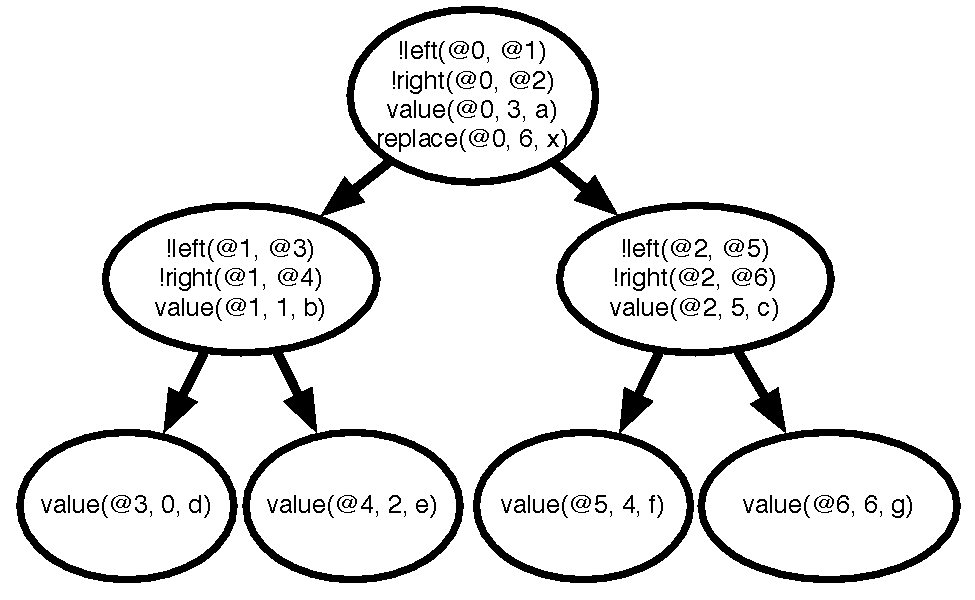
\includegraphics[width=0.44\textwidth]{figures/btree_trace1.pdf}}
\subfigure[After applying rule 3 at node $@0$]
   {\label{fig:btree_trace2}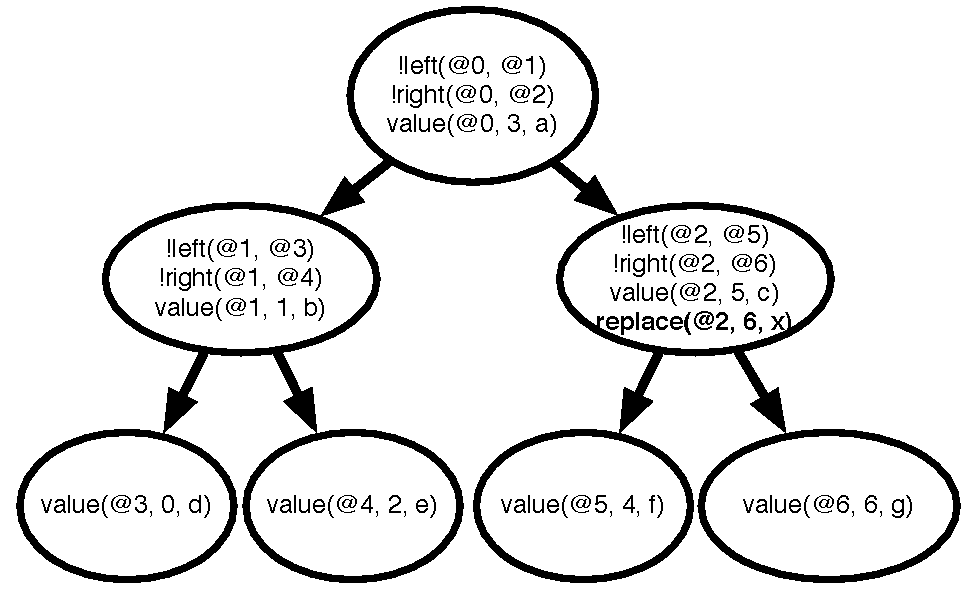
\includegraphics[width=0.44\textwidth]{figures/btree_trace2.pdf}}
\subfigure[After applying rule 3 at node $@2$]
   {\label{fig:btree_trace3}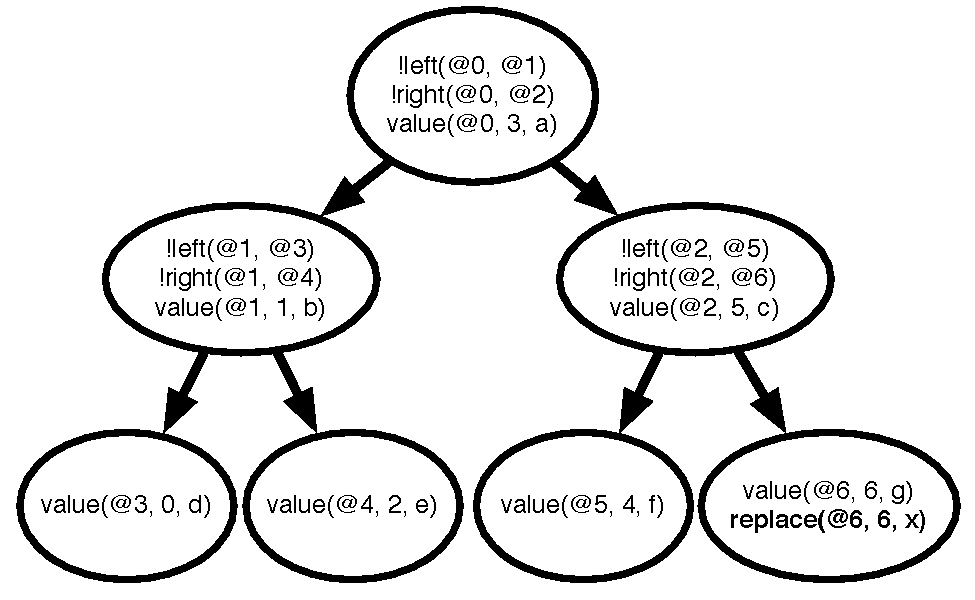
\includegraphics[width=0.44\textwidth]{figures/btree_trace3.pdf}}
\subfigure[After applying rule 1 at node $@6$]
   {\label{fig:btree_trace4}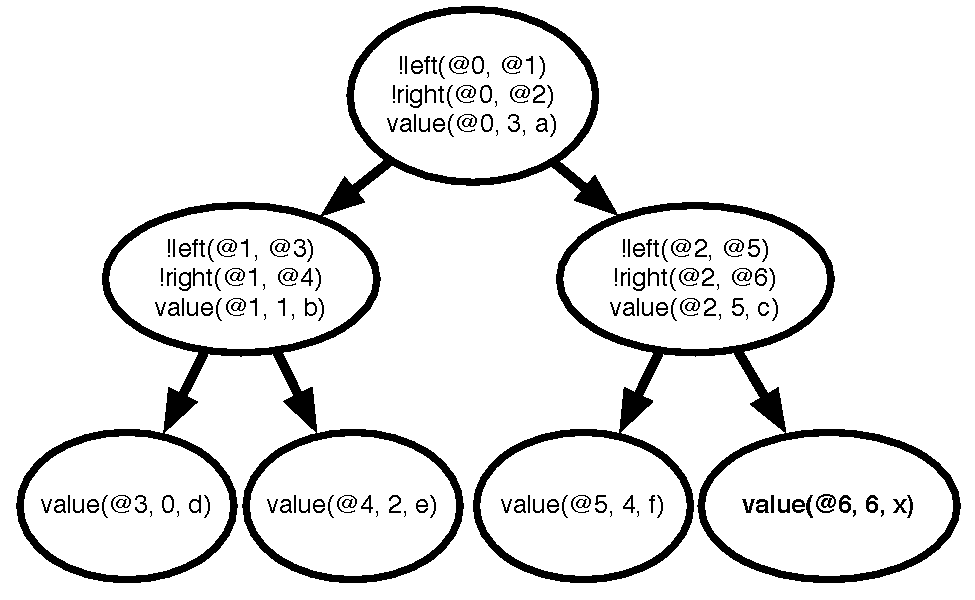
\includegraphics[width=0.44\textwidth]{figures/btree_trace4.pdf}}
\caption{An execution trace for the binary tree dictionary program}
\label{fig:btree_trace}
\end{figure*}

Figure~\ref{fig:btree_trace} illustrates the trace of the
execution. Note that the program database is partitioned by the tree
nodes using the first argument of each fact. In
Fig.~\ref{fig:btree_trace1}, we present the database filled with the
program's axioms. Next, we follow the right branch using rule 3 since
$6 > 3$ (Fig.~\ref{fig:btree_trace2}). We then use the same rule
again in Fig.~\ref{fig:btree_trace3} where we finally reach the key
6. Here, we apply rule 1 and \texttt{value(@6, 6, g)} is updated to
\texttt{value(@6, 6, x)} (Fig.~\ref{fig:btree_trace4}).

%%%%%%%%%%%%%%%%%%%%%%%%%%%%%%%%%%%%%%%%%%%%%%%%%%%%%%%%%%%%%%%%%%%%%%

\subsection{Syntax}

Table~\ref{tbl:ast} shows the abstract syntax for rules in LM.  An LM
program $Prog$ consists of a set of derivation rules $\Sigma$ and a
database $D$.  Each derivation rule $R$ can be written as $BE \lolli
HE$ where $BE$ is the body of a rule and $HE$ is the head. Rules
without bodies are allowed in LM and they are called
\textit{axioms}. Rules without heads are also allowed.  The body of a
rule, $BE$, may contain linear ($L$) and persistent ($P$) \emph{fact
  expressions} and constraints ($C$). Fact expressions are template
facts that instantiate variables (from facts in the
database). Variables can be used again in the body for matching and
also in the head when instantiating facts. Constraints are boolean
expressions that must be true in order for the rule to be
fired. Constraints use variables from fact expressions and are built
using a small functional language that includes mathematical
operations, boolean operations, external functions and literal values.
The head of a rule, $HE$, contains linear ($L$) and persistent ($P$)
\emph{fact templates} which are uninstantiated facts to derive new
facts. Head expressions may use the variables instantiated in the
body. The head can also have \emph{comprehensions} ($CE$) and
\emph{aggregates} ($AE$).

\begin{table}[ht]
\centering
{\scriptsize
\begin{tabular}{llcl}
Program          & $Prog$ & $::=$ & $\Sigma, D$ \\
Set of Rules     & $\Sigma$ & $::=$ & $\cdot \; | \; \Sigma, R$\\
Database         & $D$ & $::=$ & $\Gamma; \Delta$ \\
Rule             & $R$ & $::=$ & $BE \lolli HE \; | \; \forall_{x}. R$ \\
Body Expression  & $BE$ & $::=$ & $L \; | \; P \; | \; C \; | \; BE, BE \; | \; \exists_{x}. BE \; | \; 1$\\
Head Expression  & $HE$ & $::=$ & $L \; | \; P \; | \; HE, HE \; | \; CE \; | \; AE \; | \; 1$\\
Linear Fact      & $L$ & $::=$ & $l(\hat{x})$\\
Persistent Fact  & $P$ & $::=$ & $\bang p(\hat{x})$\\
Constraint       & $C$ & $::=$ & $c(\hat{x})$ \\
Comprehension    & $CE$ & $::=$ & $\comprehension$ \\
Aggregate        & $AE$ & $::=$ & $\aggregate$ \\
Operations       & $A$ & $::=$ & $\mathtt{min} \; | \; \mathtt{max} \; | \; \mathtt{sum} \; | \; \mathtt{count}$ \\
Sub-Head         & $SH$ & $::=$ & $L \; | \; P \; | \; SH, SH \; | \; 1$\\
Linear Facts     & $\Delta$ & $::=$ & $\cdot \; | \; \Delta, l(\hat{t})$ \\
Persistent Facts & $\Gamma$ & $::=$ & $\cdot \; | \; \Gamma, \bang p(\hat{t})$ \\
\end{tabular}
}
\caption{Abstract syntax of LM}
\label{tbl:ast}
\end{table}

We created the concept of comprehensions to be used when the
consumption of a linear fact should generate a set of facts
accordingly to the current contents of the database. In a
comprehension $\comprehension$, $\widehat{x}$ is a list of variables,
$BE$ is the body of the comprehension and $SH$ is the head. The body
$BE$ is used to generate all possible combinations for the head $SH$,
according to the facts in the database. The following program shows a
simple example that uses comprehensions:

{\footnotesize
\begin{Verbatim}
!edge(@1, @2).   !edge(@1, @3).
iterate(@1).

iterate(A)
   -o {B | !edge(A, B) | perform(B)}.
\end{Verbatim}
}

When the rule is fired, we consume \texttt{iterate(@1)} and then
generate the comprehension. Here, we iterate through all the
\texttt{edge/2} facts that match \texttt{!edge(@1, B)}, which are
\texttt{!edge(@1, @2)} and \texttt{!edge(@1, @3)}. For each fact, we
then derive \texttt{perform(B)}, namely \texttt{perform(@2)} and
\texttt{perform(@3)} in this example.

Another useful feature is the ability to reduce several facts into a
single fact. For that, we have aggregates, a special kind of sub-rule
that works very similarly to comprehensions. In a aggregate
$\aggregate$, $A$ is the aggregate operation, $\widehat{x}$ is the
list of variables introduced in $BE$, $SH_1$ and $SH_2$ and $y$ is the
variable in the body $BE$ that represents the values to be aggregated
using $A$. Like comprehensions, we use $\widehat{x}$ to try all the
combinations of $BE$, but, in addition to deriving $SH_1$ for each
combination, we aggregate the values represented by $y$ and derive
$SH_2$ only once using $y$. As an example, consider the following
program:

{\footnotesize
\begin{Verbatim}
price(@1, 3).   price(@1, 4).   price(@1, 5).
count-prices(@1).

count-prices(A)
   -o [sum => P | . | price(A, P) | 1 | total(A, P)].
\end{Verbatim}
}

By applying the rule, we consume \texttt{count-prices(@1)} and derive
the aggregate which consumes all the \texttt{price(@1, P)} linear
facts. These are summed up and \texttt{total(@1,~12)} is derived. LM
provides several aggregate operations, including the \emph{minimum},
\emph{maximum}, \emph{sum} and \emph{count}.

%%%%%%%%%%%%%%%%%%%%%%%%%%%%%%%%%%%%%%%%%%%%%%%%%%%%%%%%%%%%%%%%%%%%%%

\subsection{Concurrency}

LM is at its core a concurrent programming language. The database of
facts can be seen as a graph data structure where each node contains a
fraction of the database.  To accomplish this, we force the first
argument of each predicate to be typed as a \emph{node}. We then
restrict the derivation rules to only manipulate facts belonging to a
single node.  However, the expressions in the head may refer to other
nodes, as long as those nodes are instantiated in the body of the
rule.

Due to the restrictions on LM rules, nodes are able to run rules
independently without using other node's facts. Node computation
follows a \emph{don't care} or \emph{committed choice} non-determinism
since any node can be picked to run as long as it contains enough
facts to fire a derivation rule.  Facts coming from other nodes will
arrive in order of derivation but may be considered partially and
there is no particular order among the neighborhood. To improve
concurrency, the programmer is encouraged to write rules that take
advantage of the non-deterministic nature of execution.
